\documentclass{article}
\usepackage{amsmath}
\usepackage{graphicx}
\begin{document}
\section{Introduction}
\begin{enumerate}
\item \textbf{Overall goal } The accurate and stable evaluation of the parameter gradient of the energy expectation value, $\frac{\partial E}{\partial p}$, is an integral component of variational Monte Carlo (VMC) wave function optimization techniques.

\item \textbf{Barrier to achieving that goal } The naive MC estimate of $\frac{\partial E}{\partial p}$, while unbiased, has an infinite variance.

\item \textbf{Current state of the art} Current finite variance estimation techniques involve complicated guiding or auxiliary wave functions, such as a reweighting scheme \cite{Attaccalite2008, Avella} or the improved estimators of Assaraf and Caffarel \cite{doi:10.1063/1.1286598, Assaraf2003}.

\item \textbf{Our advancement to the state of the art } We derive and test a simple regularized estimator for $\frac{\partial E}{\partial p}$ which has finite variance, can be extrapolated to zero bias, and does not rely on guiding wave functions.
\end{enumerate}

\section{Regularized estimator}
\begin{enumerate}
\item The naive Monte Carlo estimator for $\frac{\partial E}{\partial p}$ suffers from an infinite variance due to a $1/x^4$ divergence of $Q^2$ near the nodes of $\Psi$, where $Q = \frac{H\Psi}{\Psi}\frac{\partial_p \Psi}{\Psi}$ and $x$ is the normal coordinate to the node.

\item Regularizing the naive Monte Carlo estimator for $Q$ by a function $f_\epsilon$ yields a finite variance estimation of $\frac{\partial E}{\partial p}$, where 
\[ f_\epsilon(x) = \begin{cases} 
      O(\frac{x}{\epsilon}) & \frac{x}{\epsilon} < 1 \\
      1 & \frac{x}{\epsilon} \ge 1 \\
   \end{cases}
\]

\item For a general function $f_\epsilon$ satisfying the conditions above, the regularized estimator $Q * f_\epsilon$ will result in a linear-order biased estimation of $\frac{\partial E}{\partial p}$.

\item A simple normalization condition on $f_\epsilon$ ensures a bias of $O(\epsilon^3)$, allowing for efficient extrapolation to zero bias.

\item The final conditions of continuity and smoothness of $f_\epsilon$ reduce the magnitude of this bias.

\item The finite variance, zero bias, extrapolated estimation for $\frac{\partial E}{\partial p}$ using $Q * f_\epsilon$ can be carried out in four steps.

\end{enumerate}

\section{Application to LiH molecule}
\begin{enumerate}
\item We test the effectiveness of the regularized estimator in evaluating $\frac{\partial E}{\partial p}$ for the determinantal coefficients of a multi-Slater Jastrow (MSJ) wave function for the LiH molecule.

\item Figure 1 illustrates how the regularized estimator removes the divergence of the naive estimator for $Q$ across the nodes of $\Psi$.

\item The predicted $O(1/\epsilon), O(\epsilon^3)$ scalings of the variance and bias are seen by integrating across the node, as shown in Figure 2. 

\item In Figure 3 we demonstrate the zero bias, finite-variance extrapolation for $\partial E/\partial p$ using the regularized estimator.
\end{enumerate}

\section{Conclusions}
\begin{enumerate}
\item Integral to the reliability of variational Monte Carlo wave function optimization methods is the finite variance estimation of $\frac{\partial E}{\partial p}$.

\item  In this work, we derive and test a simple regularized estimator for $\frac{\partial E}{\partial p}$ which has finite variance, can be extrapolated to zero bias, and does not rely on guiding wave functions.
\end{enumerate}

\bibliographystyle{unsrt}
\bibliography{pgradregr}

\section{Figures}
\begin{figure*}
\centering
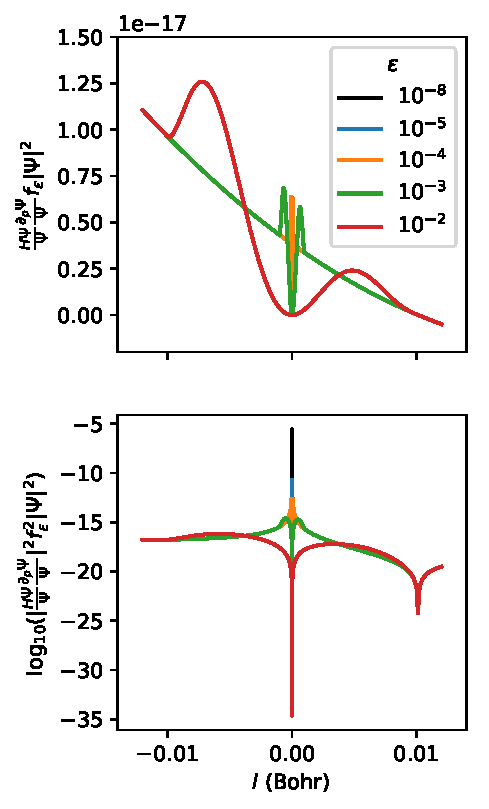
\includegraphics{../plots/viznode.pdf}
\caption{$Q * f_\epsilon$ and logarithm $(Q * f_\epsilon)^2$, $Q = \frac{H\Psi}{\Psi}\frac{\partial_p \Psi}{\Psi}$,  plotted against the normal coordinate $x$ from a node of $\Psi$. Curve colors correspond to different values of $\epsilon$ ranging from $10^{-1}$ to $10^{-8}$ Bohr.}
\end{figure*}

\begin{figure*}
\centering
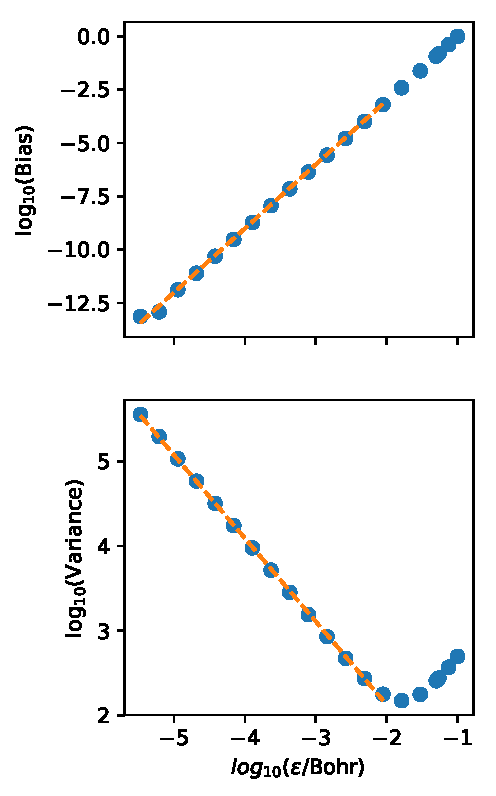
\includegraphics{../plots/integratenode.pdf}
\caption{Scaled bias and variance of Q evaluated by numerical integration from $r = -0.1$ to $r = 0.1$ across the node in Figure 1. The blue dots are the numerically integrated values and the orange curves indicate best fits to the functions $a\epsilon^3$ and $b + c/\epsilon$ for the bias and variance, respectively.}
\end{figure*}

\begin{figure*}
\centering
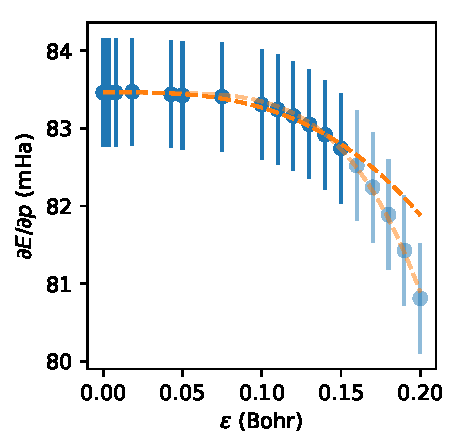
\includegraphics{../plots/dedp.pdf}
\caption{Zero bias, finite variance extrapolation for $\partial E/\partial p$ using the regularized estimator. The blue points are evaluated using VMC, the orange curve is a fit to $a + b\epsilon^3$, and the red star denotes the extrapolated estimation. }
\end{figure*}

\end{document}